\let\negmedspace\undefined
\let\negthickspace\undefined
\documentclass[journal,12pt,onecolumn]{IEEEtran}
\usepackage[margin=2.5cm]{geometry} 
\usepackage{cite}
\usepackage{amsmath,amssymb,amsfonts,amsthm}
\usepackage{algorithmic}
\usepackage{graphicx}
\graphicspath{{./figs/}}
\usepackage{textcomp}
\usepackage{xcolor}
\usepackage{txfonts}
\usepackage{listings}
\usepackage{enumitem}
\usepackage{mathtools}
\usepackage{gensymb}
\usepackage{comment}
\usepackage{caption}
\usepackage[breaklinks=true]{hyperref}
\usepackage{tkz-euclide} 
\usepackage{listings}
\usepackage{gvv}  
\usepackage{gensymb}
\usepackage{multicol}
%\def\inputGnumericTable{}                                    
\usepackage{xparse}
\usepackage{color}                                            
\usepackage{array}                                            
\usepackage{longtable}                                       
\usepackage{calc}                                             
\usepackage{multirow}
\usepackage{multicol}
\usepackage{hhline}                                           
\usepackage{ifthen}                                           
\usepackage{lscape}
\usepackage{tabularx}
\usepackage{array}
\usepackage{float}
\newtheorem{theorem}{Theorem}[section]
\newtheorem{problem}{Problem}
\newtheorem{proposition}{Proposition}[section]
\newtheorem{lemma}{Lemma}[section]
\newtheorem{corollary}[theorem]{Corollary}
\newtheorem{example}{Example}[section]
\newtheorem{definition}[problem]{Definition}
\newcommand{\BEQA}{\begin{eqnarray}}
\newcommand{\EEQA}{\end{eqnarray}}
\newcommand{\define}{\stackrel{\triangle}{=}}
\theoremstyle{remark}
\newtheorem{rem}{Remark}

\begin{document}

\title{
GATE 2015 \\
CH: CHEMICAL ENGINEERING}
\author{AI25BTECH11023 - Pratik R}
\maketitle
\renewcommand{\thefigure}{\theenumi}

\begin{enumerate}
    \item Choose the most appropriate word from the options given below to complete the following sentence.

    The principal presented the chief guest with a \rule{40pt}{0.1mm}, as token of appreciation.

\hfill{\brak{\text{GATE CH 2015}}}
\begin{enumerate}
        \item momento
         \item memento
          \item momentum
           \item moment
\end{enumerate}

    \item Choose the appropriate word/phrase, out of the four options given below, to complete the following sentence:

    Frogs \rule{40pt}{0.1mm}.

\hfill{\brak{\text{GATE CH 2015}}}
\begin{enumerate}
    \item croak
     \item roar
      \item hiss
       \item patter
\end{enumerate}

    \item Choose the word most similar in meaning to the given word:

    Educe

\hfill{\brak{\text{GATE CH 2015}}}
\begin{enumerate}
    \item Exert
     \item educate
      \item Extract
       \item Extend
\end{enumerate}

    \item Operator $\square , \diamond$ and $\to$ are defined by: $a \square b = \frac{a-b}{a+b}$; $a \diamond b = \frac{a+b}{a-b}$; $a \to b = ab$.

    Find the value of $\brak{66\square 6}\to \brak{66\diamond 6}$.

\hfill{\brak{\text{GATE CH 2015}}}
    \begin{enumerate}
        \item -2
         \item -1
          \item 1
           \item 2
    \end{enumerate}

    \item If $ \log_{x}\brak{5/7} = -1/3$, then the value of x is

\hfill{\brak{\text{GATE CH 2015}}}
\begin{enumerate}
    \item 343/125
     \item 125/343
      \item -25/49
       \item -49/25
\end{enumerate}

    \item The following question presents a sentence, part of which is underlined. Beneath the sentence you find four ways of phrasing the underlined part. Following the requirements of the standard written English, select the answer that produces the most effective sentence.
    Tuberculosis, together with its effects, ranks one of the leading causes of death in India.

\hfill{\brak{\text{GATE CH 2015}}}
\begin{enumerate}
    \item ranks as one of the leading causes of death
     \item rank as one of the leading causes of death
      \item has the rank of one of the leading causes of death
       \item are one of the leading causes of death
\end{enumerate}

    \item Read the following paragraph and choose the correct statement.
    
Climate change has reduced human security and threatened human well being. An ignored reality 
of human progress is that human security largely depends upon environmental security. But on the 
contrary. human progress seems contradictory to environmental security. To keep up both at the 
required level is a challenge to be addressed by one and all. One of the ways to curb the climate change may be suitable scientific innovations. while the other may be the Gandhian perspective on small scale progress with focus on sustainability.
change may be suitable scientific innovations. while the other may be the Gandhian perspective on small scale progress with focus on sustainability.
small scale progress with focus on sustainability.

\hfill{\brak{\text{GATE CH 2015}}}
\begin{enumerate}
    \item Human progress and security are positively associated with environmental security.
     \item Human progress is contradictory to environmental security
      \item Human security is contradictory to environmental security.
       \item Human progress depends upon environmental security.
\end{enumerate}

    \item Fill in the missing value

\hfill{\brak{\text{GATE CH 2015}}}
\begin{figure}[H]
    \centering
    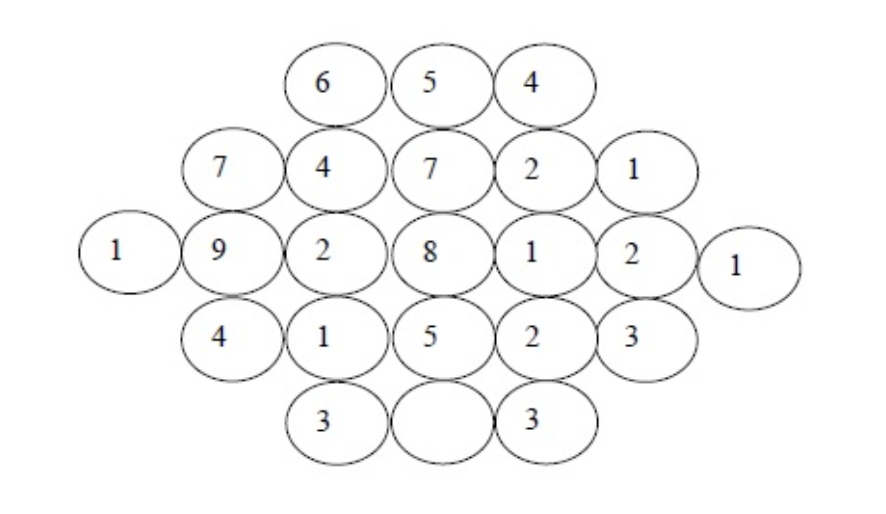
\includegraphics[width=0.5\columnwidth]{figs/8.png}
    \caption{}
    \label{fig:8}
\end{figure}

    \item A cube of side 3 units is formed using a set of smaller cubes of side 1 unit. Find the proportion of the number of faces of the smaller cubes visible to those which are NOT visible.

\hfill{\brak{\text{GATE CH 2015}}}
\begin{enumerate}
    \item 1:4
     \item 1:3
      \item 1:2
       \item 2:3
\end{enumerate}

    \item Humpty Dumpty sits on a wall every day while having lunch. The wall sometimes breaks. A person sitting on the wall falls if the wall breaks. 

Which one of the statements below is logically valid and can be inferred from the above sentences?

\hfill{\brak{\text{GATE CH 2015}}}
\begin{enumerate}
    \item Humpty Dumpty always falls while having lunch
     \item Humpty Dumpty does not fall sometimes while having lunch
      \item Humpty Dumpty never falls during dinner
       \item When Humpty Dumpty does not sit on the wall. the wall does not break 
\end{enumerate}

    \item The following set of three vectors

    \begin{align*}
        \myvec{
        1 \\
        2 \\
        1 \\
        },
        \myvec{
        x \\
        6 \\
        x \\
        } and 
        \myvec{
        3 \\
        4 \\
        2 \\
        }
    \end{align*}

is linearly dependent when x is equal to 

\hfill{\brak{\text{GATE CH 2015}}}
\begin{enumerate}
    \item 0
     \item 1
      \item 2
       \item 3
\end{enumerate}

    \item For the matrix $\myvec{
    4 & 3 \\
    3 & 4 \\
    }$, if $\myvec{
    1 \\
    1 \\
    }$ is an eigenvector, the corresponding eigenvalues is \rule{40pt}{0.1mm}.

\hfill{\brak{\text{GATE CH 2015}}}
    \item Consider a linear ordinary differential equation: $\frac{dy}{dx} + p\brak{x}y = r\brak{x}$. Functions $p\brak{x}$ and $r\brak{x}$ are defined and have a continuous first derivative. The integrating factor of this equation is non-zero. Multiplying this equation by its integrating factor converts this into a:

\hfill{\brak{\text{GATE CH 2015}}}
\begin{multicols}{2}
\begin{enumerate}
    \item Homogeneous differential equation
     \item Non\-linear differential equation
      \item second order differential equation
       \item Exact differential equation
\end{enumerate}
\end{multicols}

    \item A complex-valued function, $f\brak{z}$, given below is analytic in domain D:

    $f\brak{z}= u\brak{x,y} + iv\brak{x,y}$
    $z= x+iy$

    Which of the following is NOT correct?

\hfill{\brak{\text{GATE CH 2015}}}
\begin{enumerate}
    \item $\frac{df}{dz} = \frac{\partial v}{\partial y}+ i\frac{\partial u}{\partial y}$
    \item $\frac{df}{dz} = \frac{\partial u}{\partial x}+ i\frac{\partial v}{\partial x} $
    \item $\frac{df}{dz} = \frac{\partial v}{\partial y}- i\frac{\partial u}{\partial y} $
    \item $\frac{df}{dz} = \frac{\partial v}{\partial y}+ i\frac{\partial u}{\partial x} $
\end{enumerate}

    \item A scalar function in the xy-plane is given by $\phi \brak{x,y}= x^2  + y^2$. If $\hat{i}$ and $\hat{j}$ are unit vectors in the x and y directions, the direction of maximum increase in the value of $\phi$ at (1,1) is along:

\hfill{\brak{\text{GATE CH 2015}}}
\begin{enumerate}
    \item $-2\hat{i}+ 2\hat{j}$
     \item $2\hat{i}+ 2\hat{j}$
      \item $-2\hat{i}- 2\hat{j}$
       \item $2\hat{i}- 2\hat{j}$
\end{enumerate}

    \item For a pure liquid, the rate of change of vapour pressure with temperature is 0.1bar/K in the temperature range of 300 to 350K. if the boiling point of the liquid at 2bar is 320K, the temperature(in K) at which it will boil at 1 bar(upto one decimal place) is \rule{40pt}{0.1mm}.

\hfill{\brak{\text{GATE CH 2015}}}
    \item Three identical closed systems of a pure gas are taken from an initial temperature and pressure($T_1,P_1$) to a final state ($T_2, P_2$), each by a different path. which of the following is ALWAYS TRUE for the three systems? ($\Delta$ represents the change between the initial and final states; U, S, G, Q and W are internal energy, entropy, Gibbs free energy, heat added and work done, respectively.)

\hfill{\brak{\text{GATE CH 2015}}}
\begin{enumerate}
    \item $\Delta$U,$\Delta$S, Q are same
     \item W, $\Delta$U,$\Delta$G are same
      \item $\Delta$S, W, Q are same
       \item $\Delta$G, $\Delta$U, $\Delta$S are same
\end{enumerate}

    \item For a gas phase cracking reaction $A \to B+C$ at $300^{o}C$, the Gibbs free energy of the reaction at this temperature is $\Delta G\degree = -2750 J/mol$. The pressure is 1 bar and the gas phase can be assumed to be ideal. The universal gas constant $R = 8.314J/molK$. The fractional molar conversion of A at equilibrium is:

\hfill{\brak{\text{GATE CH 2015}}}
\begin{enumerate}
    \item 0.44
     \item 0.50
      \item 0.64
       \item 0.80
\end{enumerate}

    \item If v,u and g represent respectively the molar volume, molar internal energy, molar entropy and molar Gibbs free energy, then match the entries in the left and right columns below and choose the correct option.

\hfill{\brak{\text{GATE CH 2015}}}
\begin{multicols}{2}
    \begin{enumerate}[label =\Alph*]
        \item $-\brak{\partial u/\partial v}_s$
         \item $\brak{\partial g/\partial P}_T$
          \item $-\brak{\partial g/\partial T}_P$
           \item $\brak{\partial u/\partial s}_v$
    \end{enumerate}
\columnbreak
    \begin{enumerate}[label = \Roman*]
        \item Temperature
         \item Pressure
          \item v
           \item s
    \end{enumerate}
\end{multicols}

\begin{enumerate}
    \item A-II, B-III, C-IV, D-I 
     \item A-II, B-IV, C-III, D-I 
      \item A-I, B-IV, C-II, D-III 
       \item A-III, B-II, C-IV, D-I 
\end{enumerate}

    \item Two different liquids are flowing through different pipes of the same diameter. In the first pipe, the flow is laminar with centerline velocity, $V_{max,1}$, whereas in the second pipe, the flow is turbulent. For turbulent flow, the average velocity is 0.82 times the centerline velocity, $V_{max,2}$. For equal volumetric flow rates in both the pipes, the ratio $V_{max,1}/V_{max,2}$ (up to two decimal places) is \rule{40pt}{0.1mm}.

\hfill{\brak{\text{GATE CH 2015}}}
    \item For uniform laminar flow over a flat plate, the thickness of the boundary layer, $\delta$, at a distance $x$ from the leading edge of the plate follows the relation:

\hfill{\brak{\text{GATE CH 2015}}}
\begin{enumerate}
    \item $\delta \brak{x} \propto x^{-1}$
     \item $\delta \brak{x} \propto x$
      \item $\delta \brak{x} \propto x^{1/2}$
       \item $\delta \brak{x} \propto x^{-1/2}$
\end{enumerate}

    \item A cylinderical packed bed of height 1m is filled with equal sized spherical particles. The particles are nonporous and have a density of $1500 kg/m^3$. The void fraction of the bed is 0.45. The bed is fluidized using air (density $1kg/m^3$). If the acceleration due to gravity is $9.8 ms^2$, the pressure drop(in Pa) across the bed at incipient fluidization (up to one decimal place) is \rule{40pt}{0.1mm}.

\hfill{\brak{\text{GATE CH 2015}}}
    \item Two infinitely large parallel plates(I and II) are held at temperatures $T_1$ and $T_II$ ($T_1 > T_{II}$) respectively, and placed at a distance 2d apart in vacuum. An infinitely large flat radiation shield (III) is placed in parallel in between I and II. The emissivities of all the plates are equal. the ratio of the steady state radiative heat fluxes with and without the shield is:

\hfill{\brak{\text{GATE CH 2015}}}
\begin{figure}[H]
    \centering
    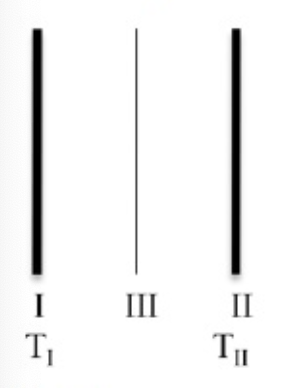
\includegraphics[width=0.25\linewidth]{figs/23.png}
    \caption{}
    \label{fig:23}
\end{figure}

\begin{enumerate}
    \item 0.5
     \item 0.75
      \item 0.25
       \item 0
\end{enumerate}

    \item For a binary mixture of components A and B, $N_A$ and $N_B$ denote the total molar fluxes of component A and B, respectively. $J_A$ and $J_B$ are the corresponding molar diffusive fluxes. Which of the following is true for equimolar counter-diffusion in the binary mixture?

\hfill{\brak{\text{GATE CH 2015}}}
\begin{enumerate}
    \item $N_A + N_B = 0$ and $J_A + J_B \neq 0$
     \item $N_A + N_B \neq 0$ and $J_A + J_B = 0$
      \item $N_A + N_B \neq 0$ and $J_A + J_B \neq 0$
       \item $N_A + N_B = 0$ and $J_A + J_B = 0$
\end{enumerate}

    \item Benzene is removed from air by absorbing it in a non-volatile wash-oil at 100kPa in a counter\-current gas absorber. Gas flow rate is 100mol/min, which includes 2mol/min of benzene. The flow rate of wash oil is 50 mol/min. Vapor pressure of benzene at the column conditions is 50kPa. Benzene forms an ideal solution with the wash oil and the column is operating at steady state. Gas phase can be assumed to follow ideal gas law. Neglect the change in molar flow rates of liquid and gas phases inside the column.

    For this process, the value of the absorption factor (up to two decimal places) is \rule{40pt}{0.1mm}.

\hfill{\brak{\text{GATE CH 2015}}}
    \item A spherical naphthalene ball of 2mm diameter is subliming very slowly in stagnant air at $25\degree C$. The change in the size of the ball during the sublimation can be neglected. The diffusivity of naphthalene in air at $25\degree C$ is $1.1 \times 10^{-6} m^2/s$.

    The value of mass transfer coefficient is $B \times 10^{-3} m/s$, where B(upto one decimal place) is \rule{40pt}{0.1mm}.

\hfill{\brak{\text{GATE CH 2015}}}
    \item Which of the following can change if only the catalyst is changed for a reaction system?

\hfill{\brak{\text{GATE CH 2015}}}
\begin{enumerate}
    \item Enthalpy of reaction
    \item Activation energy
    \item Free energy of the reaction
    \item Equilibrium constant
\end{enumerate}

    \item For which reaction order, the half life of the reactant is half of the full lifetime (times for 100\% conversion) of the reactant?

\hfill{\brak{\text{GATE CH 2015}}}
\begin{enumerate}
    \item Zero order
    \item Half order
    \item First order
    \item Second order
\end{enumerate}

    \item An irreversible, homogeneous reaction $A \to products$, has the rate expression:

\begin{align*}
    Rate = \frac{2C_{A}^{2} + 0.1 C_A}{1 + 50C_A}, \text{where $C_A$ is the concentration of A.}
\end{align*}

$C_A$ varies in the range $0.5 - 50 mol/m^3$.

For very high concentration of A, the reaction order tends to:

\hfill{\brak{\text{GATE CH 2015}}}
\begin{enumerate}
    \item 0
    \item 1
    \item 1.5
    \item 2
\end{enumerate}

    \item Match the output signals as obtained from four measuring devices in response to a unit step change in the input signal.

\hfill{\brak{\text{GATE CH 2015}}}
    \begin{multicols}{2}
        \begin{figure}[H]
            \centering
            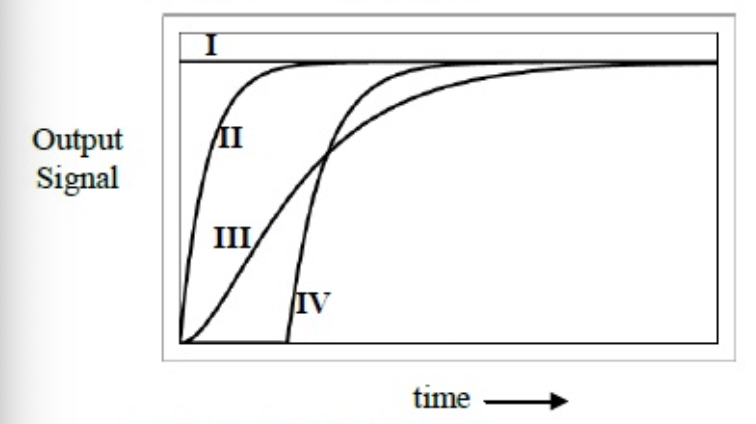
\includegraphics[width=0.7\columnwidth]{figs/30.png}
            \caption{}
            \label{fig:30}
        \end{figure}
\columnbreak
    \begin{enumerate}[label = \Alph*]
        \item Gas chromatograph, with a long capillary tube
        \item venturi tube
        \item Thermocouple with first order dynamics
        \item Pressure transducer with second order dynamics
    \end{enumerate}
    \end{multicols}

\begin{enumerate}
    \item A-IV, B-III, C-II, D-I 
     \item A-III, B-I, C-II, D-IV
      \item A-IV, B-I, C-II, D-III 
       \item A-II, B-IV, C-III, D-I 
\end{enumerate}

    \item The transfer function for the disturbance response in an open-loop process is given by $G_d^{open}\brak{s}$. The corresponding transfer function for the disturbance response in a closed-loop feedback control system with proportional controller is given by $G_d^{closed}\brak{s}$. Select the option that is ALWAYS correct $\cbrak{O\sbrak{G\brak{s}} \text{represents order of transfer function} G\brak{s}}$:

\hfill{\brak{\text{GATE CH 2015}}}
\begin{enumerate}
    \item $O\sbrak{G_d^{open}\brak{s}} = O\sbrak{G_d^{open}\brak{s}}$
     \item $O\sbrak{G_d^{open}\brak{s}} \neq O\sbrak{G_d^{open}\brak{s}}$
      \item $O\sbrak{G_d^{open}\brak{s}} \geq O\sbrak{G_d^{open}\brak{s}}$
       \item $O\sbrak{G_d^{open}\brak{s}} \leq O\sbrak{G_d^{open}\brak{s}}$  
\end{enumerate}

    \item Identify the WRONG statement amongst the following:

\hfill{\brak{\text{GATE CH 2015}}}
\begin{enumerate}
    \item Steam distillation is used for mixtures that are immiscible with water
    \item Vacuum distillation is used for mixtures that are miscible with water.
    \item Steam distillation is used for mixtures that are miscible with water
    \item Vacuum distillation columns have larger diameters as compared to atmospheric columns for the same throughput. 
\end{enumerate}

    \item Match the polymer mentioned on the left with the catalyst used for its manufacture given on the right.

\hfill{\brak{\text{GATE CH 2015}}}
\begin{multicols}{2}
    \begin{enumerate}[label = \Roman*]
        \item Low density Polyethylene
        \item High density Polyethylene
        \item Polyethylene Terephthalate
        \item Polyvinyl Chloride 
    \end{enumerate}
\columnbreak
\begin{enumerate}[label = \Alph*]
    \item Ziegler-Natta catalyst
    \item Traces of Oxygen
    \item Butyl Lithium
    \item Antimony 
\end{enumerate}
\end{multicols}

\begin{enumerate}
    \item I-Q, II-R, III-S, IV-P
     \item I-S, II-P, III-Q, IV-R
      \item I-Q, II-P, III-S, IV-R
       \item I-S, II-R, III-P, IV-Q
\end{enumerate}

    \item Match the technologies in Group 1 with the entries in Group 2:

\hfill{\brak{\text{GATE CH 2015}}}
\begin{multicols}{2}
    \begin{enumerate}[label =\Alph*]
        \item Urea manufacture
         \item Coal gasification
          \item Controlled release of chemicals
           \item Deep hydrodesulphurization
    \end{enumerate}
\columnbreak
    \begin{enumerate}[label = \Roman*]
        \item Microencapsulation
         \item Ultra-low sulphur diesel
          \item Shale oil
           \item Prilling tower
           \item Gas hydrates
           \item Gas solid non catalytic reaction
    \end{enumerate}
\end{multicols}

\begin{enumerate}
    \item A-I, B-V, C-II, D-VI 
     \item A-IV, B-VI, C-I, D-II
      \item A-IV, B-I, C-III, D-II 
       \item A-V, B-VI, C-IV, D-II
\end{enumerate}

    \item Match the chemicals written on the left with raw materials required to produce them mentioned on the right.

\hfill{\brak{\text{GATE CH 2015}}}
\begin{multicols}{2}
    \begin{enumerate}[label =\Roman*]
        \item Single Superphosphate
         \item Triple Superphosphate
          \item Diammonium Phosphate
           \item Caustic soda
    \end{enumerate}
\columnbreak
    \begin{enumerate}[label = \Alph*]
        \item Rock phosphate + Sulphuric Acid + Ammonia
         \item Brine
          \item Rock phosphate + Sulphuric Acid
           \item Rock phosphate + Phosphoric Acid
    \end{enumerate}
\end{multicols}

\begin{enumerate}
    \item I-Q, II-R, III-S, IV-P
     \item I-S, II-P, III-Q, IV-R
      \item I-R, II-S, III-P, IV-Q
       \item I-S, II-R, III-P, IV-Q
\end{enumerate}    

    \item The diameters of sand particles in a sample range from 50 to 150 microns. The number of particles of diameter $x$ in the sample is proportional to $\frac{1}{50+x}$. The average diameter, in microns, (upto one decimal place) is \rule{40pt}{0.1mm}.

\hfill{\brak{\text{GATE CH 2015}}}
    \item A vector $u = -2y\hat{i} + 2x\hat{j}$, where $\hat{i}$ and $\hat{j}$ are unit vectors in $x$ and $y$ directions, respectively. Evaluate the line integral
    \begin{align*}
        I = \oint_{C} u \, dx
    \end{align*}

    where C is a closed loop formed by connecting points (1,1), (3,1), (3,2), (1,2) in that order. The value of I is \rule{40pt}{0.1mm}.

\hfill{\brak{\text{GATE CH 2015}}}
    \item The solution of the non linear equation 
    \begin{align*}
        x^3 - x = 0
    \end{align*}

    is to be obtained using Newton Raphson method. If the initial guess is $x = 0.5$, the method converges to which of the following values:

\hfill{\brak{\text{GATE CH 2015}}}
\begin{enumerate}
    \item -1
    \item 0
    \item 1
    \item 2
\end{enumerate}

    \item For complex variable z, the value of the contour integral $\frac{1}{2\pi \iota} \int_{C} \frac{e^{-2z}}{z\brak{z-3}} \, dz$ along the clockwise contour C: $|z| = 2$ (upto two decimal places) is \rule{40pt}{0.1mm}.

\hfill{\brak{\text{GATE CH 2015}}}
    \item The schematic diagram of a steady state process is shown below. The fresh feed(F) to the reactor consists of 96 mol\% reactant A and 4mol\% inert I. The stoichiometry of the reaction is $A \to C$. A part of the reactor effluent is recycled. The molar flow rate of the recycle stream is 0.3 F. The product stream P contains 50mol\% C. The percentage conversion of A in the reactor based on A entering the reactor at point 1  in the figure (up to one decimal place) is \rule{40pt}{0.1mm}.

\hfill{\brak{\text{GATE CH 2015}}}
    \begin{figure}[H]
        \centering
        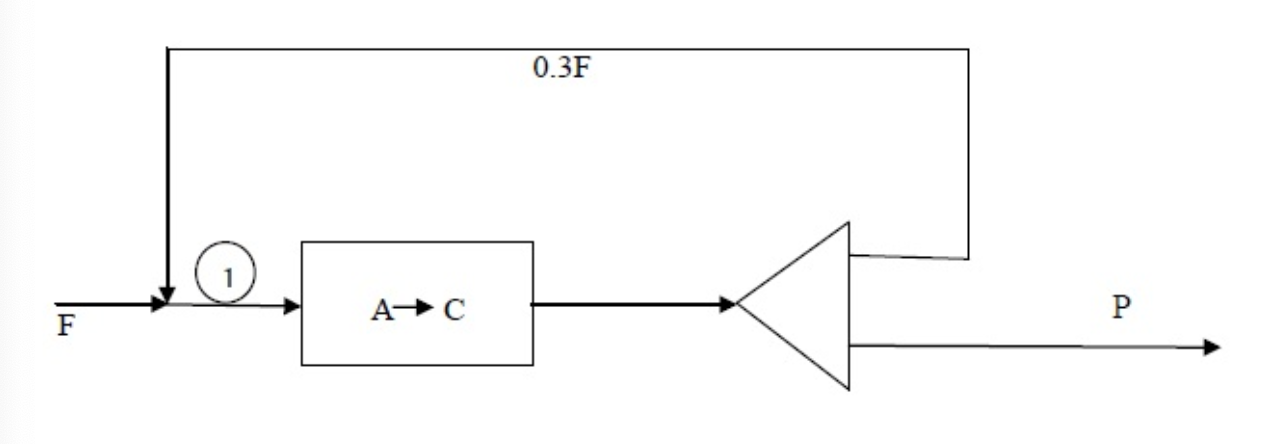
\includegraphics[width=0.5\columnwidth]{figs/40.png}
        \caption{}
        \label{fig:40}
    \end{figure}

    \item An ideal gas is initially at a pressure of 0.1 Mpa and a total volume of $2m^3$. It is first compressed to 1 Mpa by a reversible adiabatic process and then cooled at constant pressure to a final volume of $0.2m^3$. The total work done (in kJ) on the gas for the entire process (up to one decimal place) is \rule{40pt}{0.1mm}.

    Data: $R=8.314J/molK$; heat capacity at constant pressure $\brak{C_P} = 2.5R$

\hfill{\brak{\text{GATE CH 2015}}}
    \item Given that molar residual Gibbs free energy, $g^R$, and molar residual volume, $v^R$, are related as $\frac{g^R}{RT}=\int_{0}^{P}\brak{\frac{v^R}{RT}}\, dP$, find $g^R$ at $T = 27\degree C$ and $P = 0.2MPa$. The gas may be assumed to follow the virtual equation of state, $z=1+BP/RT$, where $B = -10^{-4}m^3/mol$ at the given conditions (R = 8.314 J/molK). The value of $g^R$ in J/mol is:

\hfill{\brak{\text{GATE CH 2015}}}
\begin{enumerate}
    \item 0.008
    \item -2.4
    \item 20
    \item -20
\end{enumerate}

    \item A binary mixture of components (1) and (2) forms an azeotrope at $130\degree C$ and $x_1 = 0.3$. The liquid phase non ideality is described by $\ln\gamma_2 = Ax^{2}_2$ and $\ln\gamma_1 = Ax^{1}_2$, where $\gamma_1, \gamma_2$ are the activity coefficients, and $x_1$, $x_2$ are the liquid phase mole fractions. For both components, the fugacity coefficients are 0.9 at the azeotropic composition. Saturated vapor pressure at $130\degree C$ are $P^{sat}_1=70$ bar and $P^{sat}_2= 30$ bar.

    The total pressure in bars for the above azeotropic system (up to two decimal places) is \rule{40pt}{0.1mm}.

\hfill{\brak{\text{GATE CH 2015}}}
    \item For Fanning fiction factor f(for flow in pipes) and drag coefficient $C_D$(for flow over immersed bodies), which of the following statements are true?

\hfill{\brak{\text{GATE CH 2015}}}
\begin{enumerate}[label = \Alph*]
    \item f accounts only for the skin friction
    \item $C_D$ accounts only for the form friction
    \item $C_D$ accounts for both skin friction and form friction
    \item Both f and $C_D$ depends on the Reynolds number
    \item For laminar flow through a pipe, f doubles on doubling the volumetric flow rate.
\end{enumerate}

\begin{multicols}{4}
    \begin{enumerate}
        \item C, D, E
        \item A, B, D
        \item A, C, D
        \item A, B, D, E
    \end{enumerate}
\end{multicols}

    \item A centrifugal pump delivers water at the rate of $0.22 m^3/s$ from a reservoir at ground level to another reservoir at a height $H$, through a vertical pipe of $0.2 m$ diameter. Both the reservoirs are open to atmosphere. The power input to the pump is 90 kW and it operates with an efficiency of 75/%.

    Data:
    Fanning friction factor for pipe flow is $f=0.04$. Neglect other head losses.
    Take gravitational acceleration, $g = 9.8 m/s^2$ and density of water is $1000kg/m^3$. 

    The height H, in meters, to which the water can be delivered(up to one decimal place) is \rule{40pt}{0.1mm}.

\hfill{\brak{\text{GATE CH 2015}}}
    \item A typical batch filtration cycle consists of filtration followed by washing. One such filtration unit operating at constant pressure difference first first filters a slurry during which is done for $t_W$ seconds and uses 1 liter of wash water. Assume the following relation to be applicable between the applied pressure drop $\Delta P$, cake thickness L at time t, and volume of liquid V collected in time t:

    \begin{align*}
        \frac{\Delta P}{L} = k_1 \frac{dv}{dt} ; L = k_2V, \textit{if L is changing}.
    \end{align*}

    $k_1$ and $k_2$ can be taken to be constant during filtration and washing. The wash time $t_w$, in seconds (up to one decimal place), is \rule{40pt}{0.1mm}.

\hfill{\brak{\text{GATE CH 2015}}}
        \item A spherical solid particle of 1mm diameter is falling with a downward velocity of 1.7 mm/s through a liquid(viscosity 0.04 Pa.s) at a low Reynolds number (Stokes regime). The liquid is flowing upward at a velocity of 1mm/s. All velocities are with respect to a stationary reference frame. Neglecting the wall effects, the drag force per unit projected area of the particle, in Pa, (up to two decimal places) is \rule{40pt}{0.1mm}.

\hfill{\brak{\text{GATE CH 2015}}}
\begin{figure}[H]
    \centering
    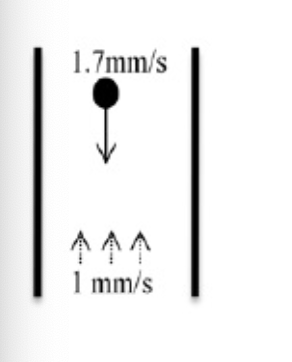
\includegraphics[width=0.5\columnwidth]{figs/47.png}
    \caption{}
    \label{fig:47}
\end{figure}

    \item In the figure below, the temperature profiles of cold and hot fluids in counter current double pipe heat exchangers(in different modes of operation) are shown on the left. For each case, match the heat exchange process for the fluid represented by the bold curve with the options given on the right.

\hfill{\brak{\text{GATE CH 2015}}}
\begin{figure}[H]
    \centering
    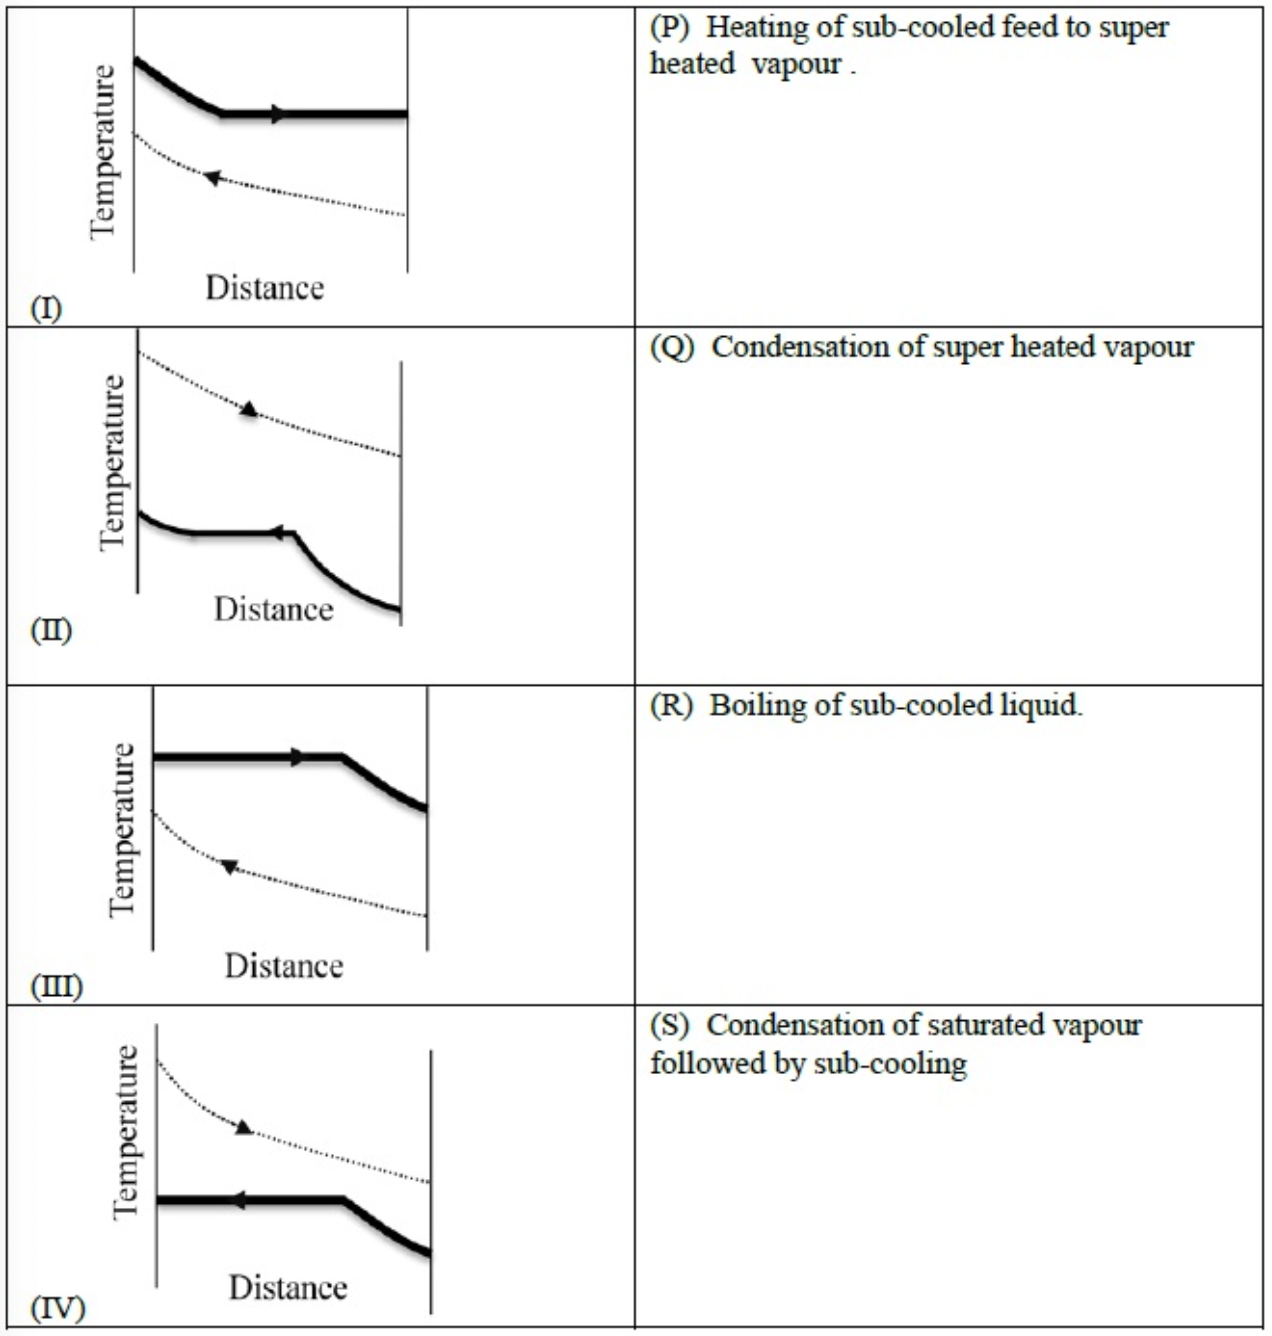
\includegraphics[width=0.5\columnwidth]{figs/48.png}
    \caption{}
    \label{fig:48}
\end{figure}

    \item A heated solid copper sphere(of surface area A and volume V) is immersed in a large body of cold fluid. Assume the resistance to heat transfer inside the sphere to be negligible and heat transfer coefficient(h), density($\rho$), heat capacity(C), and thermal conductivity(k) to be constant. Then, at time t, the temperature difference between the sphere and the fluid is proportional to:

    \hfill{\brak{\text{GATE CH 2015}}}
\begin{multicols}{2}
\begin{enumerate}
    \item $exp\sbrak{-\frac{hA}{\rho CA}t}$
    \item $exp\sbrak{-\frac{\rho V C}{hA}t}$
    \item $exp\sbrak{-\frac{4\pi k}{\rho CA}t}$
    \item $exp\sbrak{-\frac{\rho C A}{4\pi k}t}$
\end{enumerate}
\end{multicols}

    \item Air is flowing at a velocity of 3m/s perpendicular to a long pipe as shown in the figure below. The outer diameter of the pipe is $d = 6cm$ and temperature at the outside surface of the pipe is maintained at $100\degree C$. The temperature of the air far from the tube is $30\degree C$ 

    Data for air: Kinematic viscosity, $v = 18\times 10^{-6} m^2/s$; Thermal conductivity,k = 0.03 W/(mK)

    Using the Nusselt number correlation: $Nu = \frac{hd}{k} = 0.024 \times Re^{0.8}$, the rate of heat loss per unit length(W/m) from the pipe to air(up to one decimal place) is \rule{40pt}{0.1mm}.

\hfill{\brak{\text{GATE CH 2015}}}
\begin{figure}[H]
    \centering
    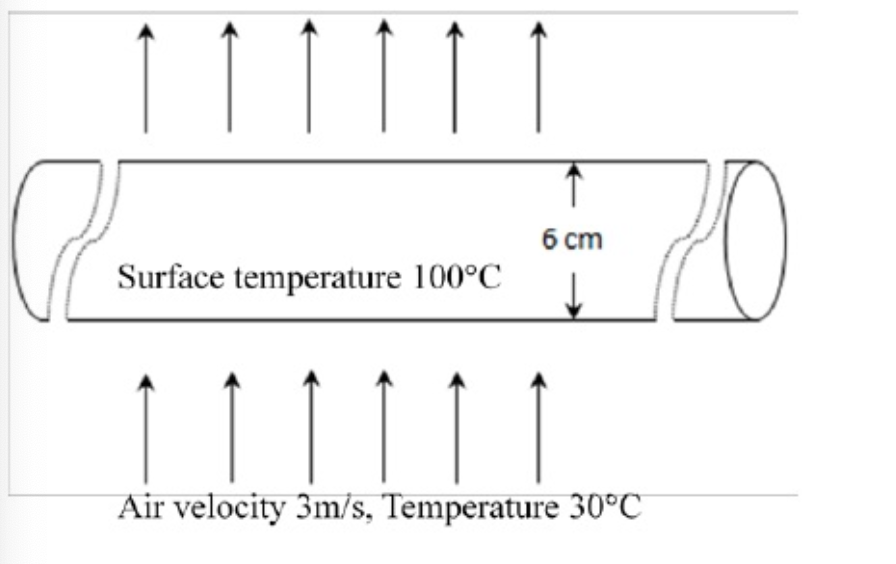
\includegraphics[width=0.5\columnwidth]{figs/50.png}
    \caption{}
    \label{fig:50}
\end{figure}

    \item Consider a solid block of unit thickness for which the thermal conductivity decreases with an increase in temperature. The opposite faces of the block are maintained at constant but different temperatures: $T\brak{x=0}>T\brak{x=1}$. Heat transfer is by steady state conduction in x direction only. There is no source or sink of heat inside the block. In the figure below, identify the correct temperature profile in the block.

\hfill{\brak{\text{GATE CH 2015}}}
\begin{figure}[H]
    \centering
    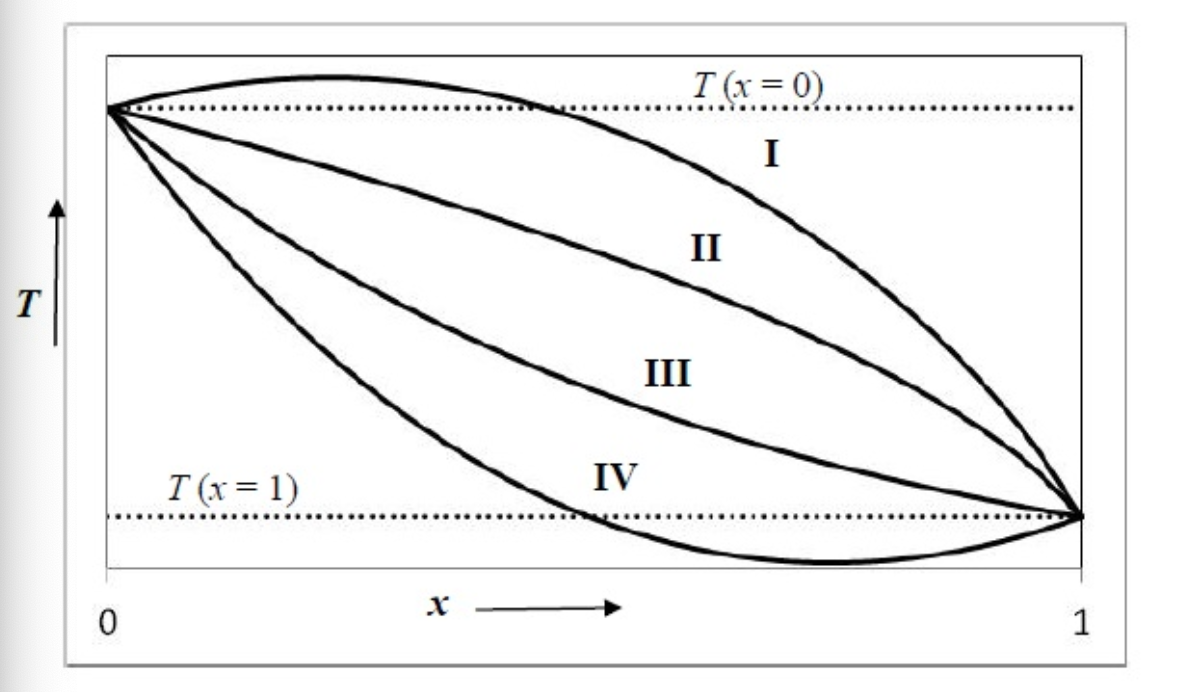
\includegraphics[width=0.5\columnwidth]{figs/51.png}
    \caption{}
    \label{fig:51}
\end{figure}

\begin{enumerate}
    \item I
    \item II
    \item III
    \item IV
\end{enumerate}

    \item A multi stage, counter current liquid liquid extractor is used to separate solute C from a binary mixture(F) of A and C using solvent B is recovered from the raffinate R by distillation, as shown in the schematic diagram below.

    \begin{figure}[H]
        \centering
        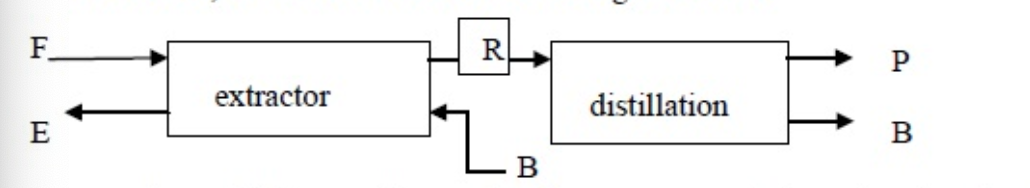
\includegraphics[width=0.5\columnwidth]{figs/52a.png}
        \caption{}
        \label{fig:52a}
    \end{figure}

    Location of different mixtures for this process are indicated on the triangular diagram below. P is the solvent free raffinate, E is the extract, F is the feed and $\Delta$ is the difference point from which the mass balance lines originate. The line PB intersects the binodal curve at U and T. The lines $P\Delta$ and FB intersects the binodal curve at V and W respectively.

    \begin{figure}[H]
        \centering
        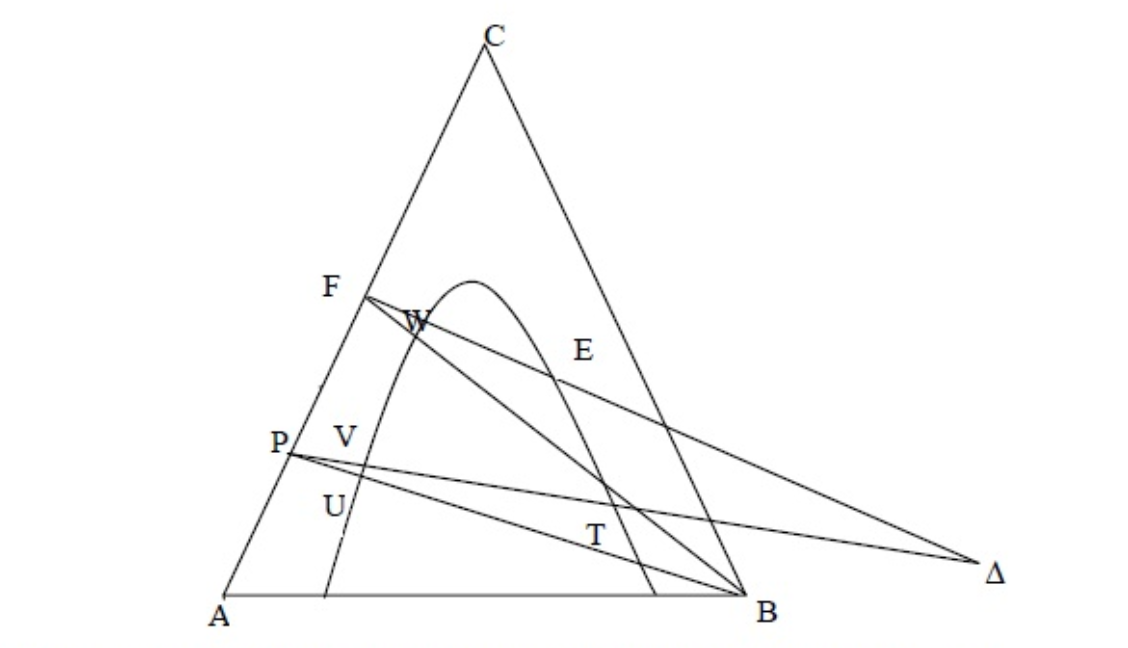
\includegraphics[width=0.5\columnwidth]{figs/52b.png}
        \caption{}
        \label{fig:52b}
    \end{figure}

The raffinate coming out of the extractor is represented in the diagram by the point:

\hfill{\brak{\text{GATE CH 2015}}}
\begin{enumerate}
    \item T
    \item U
    \item V
    \item W
\end{enumerate}

\item A binary feed consisting of 25 mol\% liquid and 75 mol\% vapour is separated in a staged distillation column. The mole fraction of the more volatile component in the distillate product is 0.95. The molar flow rate of distillate is 50\% of the feed flow rate and the McCabe\-Thiele method can be used to analyze the column. The q-line intersects the operating line of the enriching section at (0.35, 0.5) on the x\-y diagram. The slope of the stripping section operating line (up to one decimal place) is  \rule{40pt}{0.1mm}

\hfill{\brak{\text{GATE CH 2015}}}
\item Consider a steady state mass transfer process between well-mixed liquid and vapour phases of a binary mixture comprising of components A and B. The mole fractions of component A in the bulk liquid ($x_A$) and bulk vapour ($y_A$) phases are 0.36 and 0.16, respectively. The mass transfer coefficients for component A in liquid and vapour phases are $0.1mol/\brak{m^2s}$ and $0.05 mol/\brak{m^2s}$, respectively. The vapour liquid equilibrium can be approximated as $y_A = 2 x_A$, for $x_A$ less than 0.4.
The mole fraction of A in the liquid at the intrface (up to two decimal places) is \rule{40pt}{0.1mm}.

\hfill{\brak{\text{GATE CH 2015}}}
\item Adsorption on activated carbon is to be used for reducing phenol concentration in wastewater from 0.04 mol/l to 0.008 mol/l. The adsorption isotherm at the operating temperature can be expressed as $q = 0.025C^{1/3}$ ; where q is the phenol concentration in solid (mol/g solid) and C is the phenol concentration in water (mol/l). The minimum amount of solid (in grams) required per liter of wastewater (up to one decimal place) is  \rule{40pt}{0.1mm}.

\hfill{\brak{\text{GATE CH 2015}}}
\item Consider two steady isothermal flow configurations shown schematically as Case I and Case II below. In Case I, a CSTR of volume $V_1$ is followed by a PFR of volume $V_2$, while in Case II a PFR of volume $V_2$ is followed by a CSTR of volume $V_1$. In each case, a volumetric flow rate $Q$ of liquid reactant is flowing through the two units in series. An irreversible reaction $A \to products$(order n) takes place in both cases, with a reactant concentration $C_{A0}$ being fed into the first unit. 

\begin{figure}[H]
    \centering
    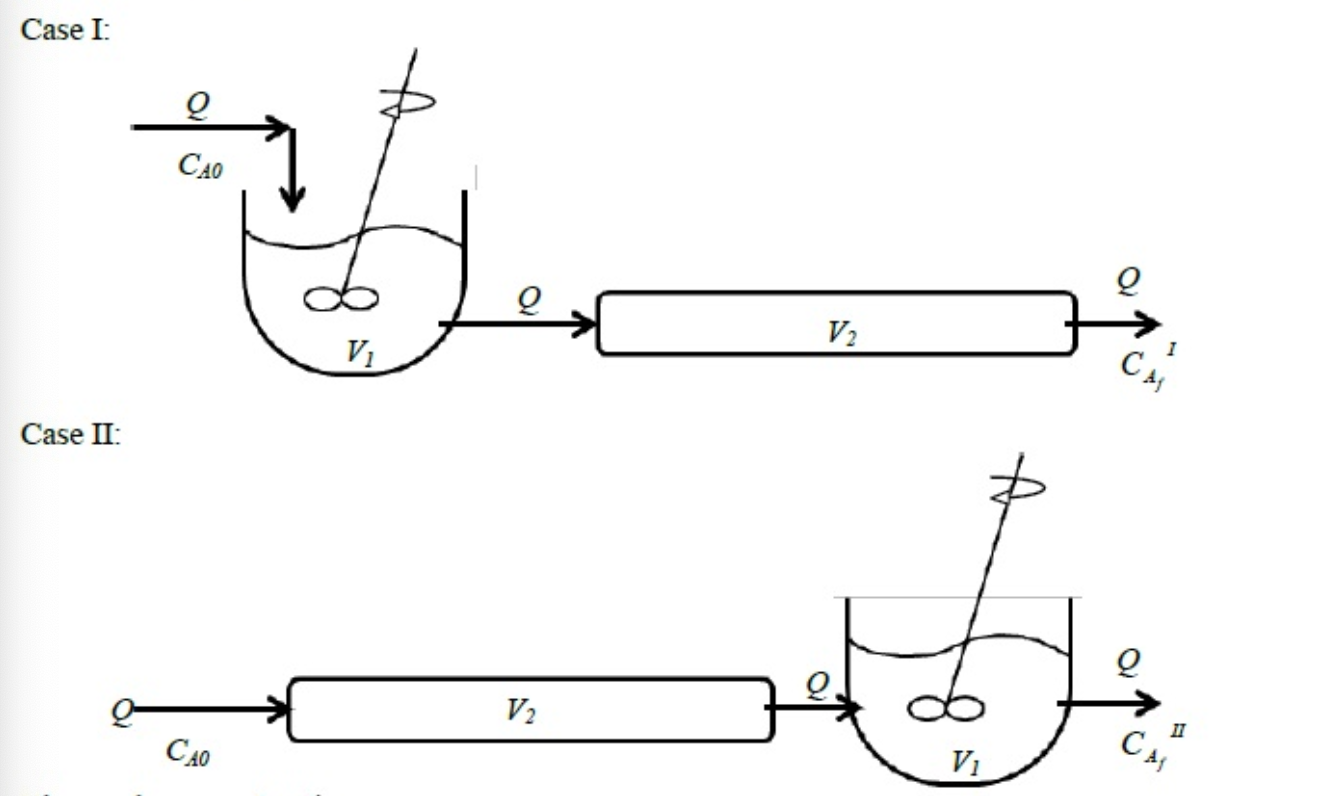
\includegraphics[width=0.5\columnwidth]{figs/56.png}
    \caption{}
    \label{fig:56}
\end{figure}

Choose the correct option:

\hfill{\brak{\text{GATE CH 2015}}}
\begin{enumerate}
    \item $\frac{C_{A_f}^{I}}{C_{A_f}^{II}} > 1$ for $n=1$
     \item $\frac{C_{A_f}^{I}}{C_{A_f}^{II}} = 1$ for $n=1$
      \item $\frac{C_{A_f}^{I}}{C_{A_f}^{II}} < 1$ for $n=1$
       \item $\frac{C_{A_f}^{I}}{C_{A_f}^{II}} = 1$ for $n>0$
\end{enumerate}

    \item A catalyst slab of half thickness L (the width and length of the $slab >> L$) is used to conduct the first order reaction $A\to B$. At 450 K, the Thiele modulus for this system is 0.5. The activation energy for the first order rate constant is 100 kJ/mol. The effective diffusivity of the reactant in the slab can be assumed to be independent of temperature, and external mass transfer resistance can be neglected. If the temperature of the reaction is increased to 470 K, then the effectiveness factor at 470 K (up to two decimal places) will be  \rule{40pt}{0.1mm}.

Value of universal gas constant = 8.314 J/mol. K. 

\hfill{\brak{\text{GATE CH 2015}}}
    \item The impulse response to a tracer pulse experiment for a flow reactor is given below:

    \begin{figure}[H]
        \centering
        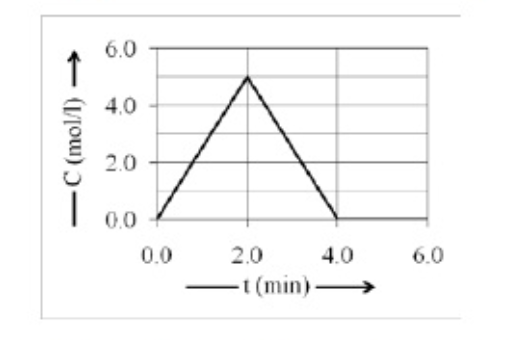
\includegraphics[width=0.5\columnwidth]{figs/58m.png}
        \caption{}
        \label{fig:58m}
    \end{figure}

In the above figure, C is the exit tracer concentration. The corresponding $E$ or $E_\theta$(normalized E) curve is correctly represented by which of the following choices? Here, $\theta $ is dimensionless time.

\hfill{\brak{\text{GATE CH 2015}}}
\begin{multicols}{2}
    \begin{enumerate}
        \item \begin{figure}[H]
            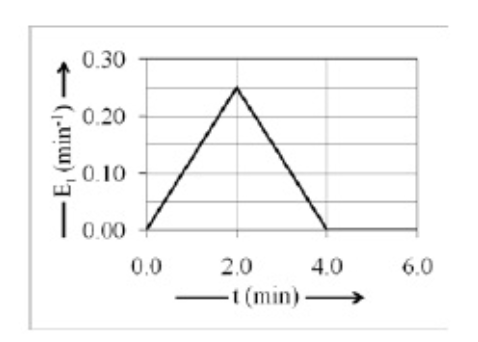
\includegraphics[width=0.5\linewidth]{figs/58a.png}
            \label{fig:58a}
        \end{figure}

         \item \begin{figure}[H]
            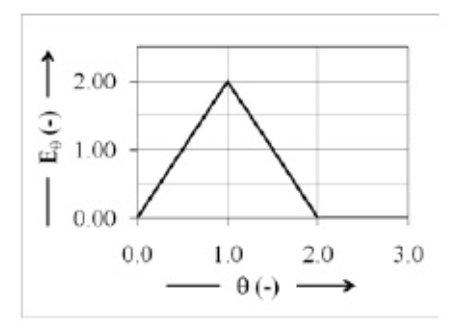
\includegraphics[width=0.5\linewidth]{figs/58b.png}
            \label{fig:58b}
        \end{figure}

         \item \begin{figure}[H]
            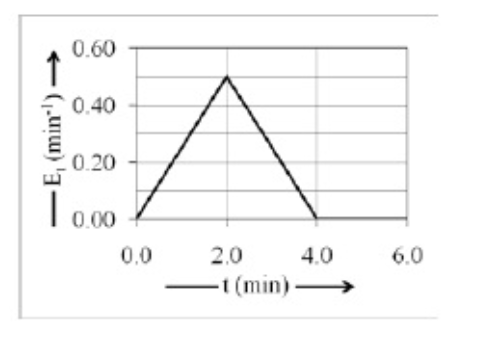
\includegraphics[width=0.5\linewidth]{figs/58c.png}
            \label{fig:58c}
        \end{figure}

         \item \begin{figure}[H]
            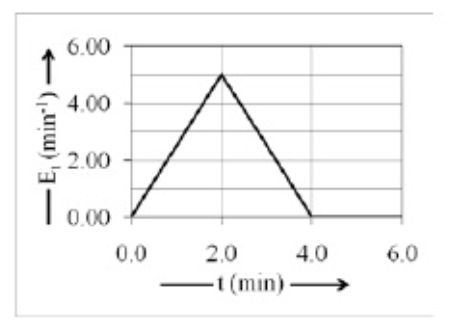
\includegraphics[width=0.5\linewidth]{figs/58d.png}
            \label{fig:58d}
        \end{figure}
    \end{enumerate}
\end{multicols}

    \item An isothermal steady state mixed flow reactor (CSTR) of $1 m^3$ volume is used to carry out the first order liquid phase reaction $A\to products$. Fresh feed at a volumetric flow rate of Q containing reactant A at a concentration $C_AO$ mixes with the recycle stream at a volumetric flow rate $RQ$ as shown in the figure below.

\hfill{\brak{\text{GATE CH 2015}}}
    \begin{figure}[H]
        \centering
        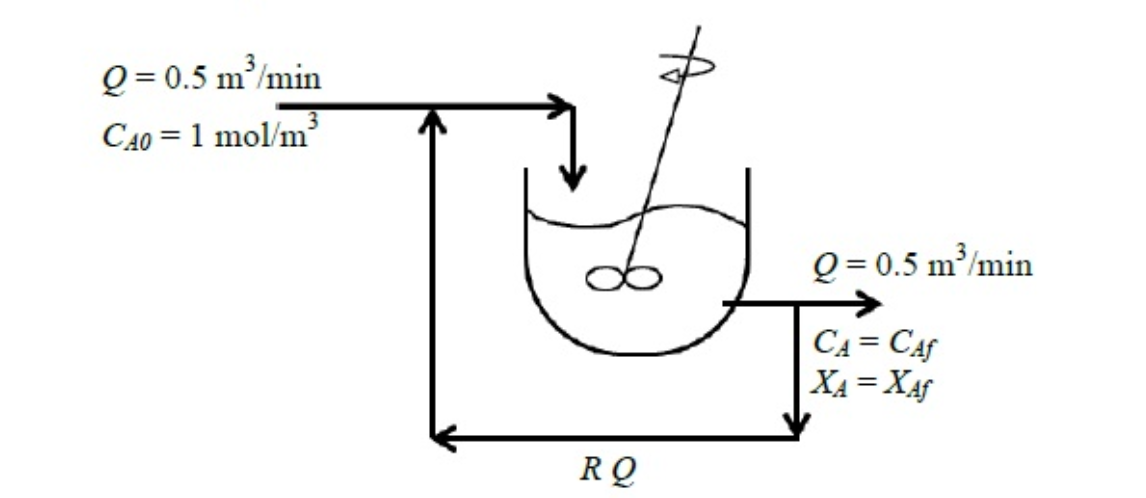
\includegraphics[width=0.5\linewidth]{figs/59.png}
        \caption{}
        \label{fig:59}
    \end{figure}

    It is observed that when the recycle ratio $R=0.5$, the exit conversion $ X_{Af}=50\% $. When the recyle ratio is increased to $R=2$, the new exit conversion(in percent) will be:

\hfill{\brak{\text{GATE CH 2015}}}
    \begin{enumerate}
        \item 50.0
        \item 54.3
        \item 58.7
        \item 63.2
    \end{enumerate}

    \item Which one of the following transfer functions, upon a unit step change in disturbance at t = 0, will show a stable time domain response with a negative initial slope (i.e., slope at t = 0):

\hfill{\brak{\text{GATE CH 2015}}}
    \begin{enumerate}
        \item $G\brak{s}=\frac{1}{s+1}- \frac{2}{s+4}$
        \item $G\brak{s}=\frac{1}{s+1}+ \frac{2}{s+4}$
        \item $G\brak{s}=\frac{1}{s+1}+ \frac{2}{s-4}$
        \item $G\brak{s}=\frac{1}{s-1}+ \frac{2}{s-4}$
    \end{enumerate}

    \item The block diagram for a process with feedback control for output deviation variable $h$ is shown in the figure below. All transfer functions are given with pre factor of $s$ in minutes. A unit step change is made in the set-point at $t=0$. The time required for h to reach 50\% of its ultimate value, in minutes (up to two decimal places), is: \rule{40pt}{0.1mm}.
    
\begin{figure}[H]
    \centering
    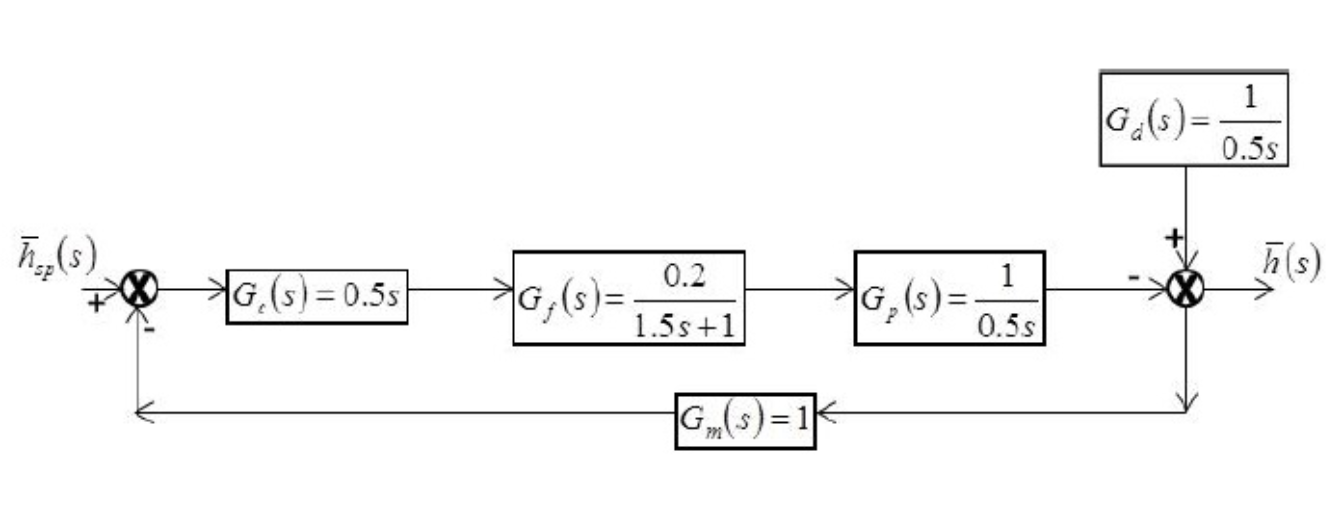
\includegraphics[width=0.5\linewidth]{figs/61.png}
    \caption{}
    \label{fig:61}
\end{figure}

Consider a control system  with the open loop transfer function given by:
\begin{align*}
    G_{OL}\brak{s}=\frac{K_ce^{-0.3s}}{1.5s+1}
\end{align*}

In the above function, pre factor of s is in minutes and $K_c$ is the gain of proportional controller. The frequency for phase margin of $30\degree $ is 4.04 rad/min. The value of $K_c$ for a gain margin of 1.7(up to one decimal place) is \rule{40pt}{0.1mm}

\hfill{\brak{\text{GATE CH 2015}}}
    \item The cost of two independent process variables $f_1$ and $f_2$ affects the total cost $C_T$ (in lakhs of rupees) of the process as per the following function:
\begin{align*}
    C_T = 100f_1 + \frac{1000}{f_1f_2} + 20f_2^{2} +50
\end{align*}

The lowest total cost $C_T$, in lakhs of rupees (up to one decimal place), is\rule{40pt}{0.1mm}.

\hfill{\brak{\text{GATE CH 2015}}}
    \item A proposed chemical plant is estimated to have a fixed capital (FC) of Rs. 24 crores. Assuming other costs to be small, the total investment may be taken to be same as FC. After commissioning (at t=0 years), the annual profit before tax is Rs. 10 crores /year (at the end of each year) and the expected life of the plant is 10 years. The tax rate is 40\% per year and a linear depreciation is allowed at 10\% per year. The salvage value is zero. If the annual interest rate is 12\%, the NPV (net present value or worth) of the project in crores of rupees (up to one decimal place) is\rule{40pt}{0.1mm}.

\hfill{\brak{\text{GATE CH 2015}}}
    \item Select the WRONG statement regarding water gas shift converters from the list below.

\hfill{\brak{\text{GATE CH 2015}}}
\begin{enumerate}
    \item Inter-stage cooling is provided between the two stages of shift converters. 
    \item Usually high temperature shift (HTS) reactor has a iron-based catalyst and low temperature shift (LTS) reactor has a copper-based catalyst.

    \item HTS reactor is followed by LTS reactor.

    \item LTS reactor is followed by HTS reactor.
\end{enumerate}
\end{enumerate}














\end{document}